\documentclass{beamer}
\mode<presentation>
{
  \usetheme{Darmstadt}
  \definecolor{BYUBlue}{RGB}{00,22,55}
  \definecolor{BYUTan}{RGB}{232,211,175}
  \usecolortheme[named=BYUBlue]{structure}
  \setbeamercolor*{palette primary}{use=structure,fg=BYUBlue,bg=lightgray}
  \setbeamercolor*{palette quaternary}{fg=white,bg=lightgray!0!BYUBlue}
  \setbeamercolor{frametitle}{fg=BYUBlue,bg=BYUBlue!10}
  \setbeamertemplate{items}[circle]
  \setbeamertemplate{blocks}[rounded][shadow=True]
  \setbeamertemplate{navigations symbols}{circle}
}

\usepackage{graphics}
\usepackage[english]{babel}
\usepackage[utf8]{inputenc}
\usepackage{times}
\usepackage{forest}
\usepackage{subfigure}
\usepackage{caption}
\captionsetup{labelformat=empty}% redefines the caption setup of the figures environment in the beamer class.
\usepackage[T1]{fontenc}
\usepackage{array}
\usepackage{amsmath,amssymb}
\usepackage{booktabs}
\usepackage{colortbl}
\usepackage{array}
\usepackage{threeparttable}
\usepackage{multirow}
\usepackage{amsthm}
\usepackage{float,graphicx,color}
\usepackage{graphics}
\usepackage{multicol}
\usepackage{natbib}
\usepackage{color}
\usepackage{hyperref}
\hypersetup{colorlinks, urlcolor=blue}
\usepackage{threeparttable}
% \usepackage[format=hang,font=normalsize,labelfont=bf]{caption}
% \usepackage{subcaption}
\usepackage{delarray}
\usepackage{amssymb}
\usepackage{setspace}
\usepackage{placeins}
\usepackage{multirow}
\usepackage{mathtools}
\usepackage{animate}
\usepackage{bm}
\usepackage{amsmath,bm}
\usepackage{amssymb}
\usepackage{amsthm}
\newtheorem*{thm}{Theorem}
\theoremstyle{definition}
\newtheorem*{defn}{Definition}
\newcommand\ve{\varepsilon}
\newcommand\norm[1]{\left\lVert#1\right\rVert}
\DeclareMathOperator*{\argmin}{argmin}

% Python code blocks --------------------------------------
\usepackage{pythonhighlight}
\usepackage{tcolorbox}
\definecolor{codegreen}{rgb}{0,0.6,0}
\definecolor{codegray}{rgb}{0.5,0.5,0.5}
\definecolor{codepurple}{rgb}{0.58,0,0.82}
\definecolor{backcolour}{rgb}{0.95,0.95,0.92}

\lstdefinestyle{mystyle}{
    backgroundcolor=\color{backcolour},
    commentstyle=\color{codegreen},
    keywordstyle=\color{magenta},
    numberstyle=\tiny\color{codegray},
    stringstyle=\color{codepurple},
    basicstyle=\ttfamily\footnotesize,
    breakatwhitespace=false,
    breaklines=true,
    captionpos=b,
    keepspaces=true,
    numbers=left,
    numbersep=5pt,
    showspaces=false,
    showstringspaces=false,
    showtabs=false,
    tabsize=2
}

\lstset{style=mystyle}


\title[OG-PHL Examples: 5-day Workshop]{OG-PHL Examples: \\ From 5-day Workshop}

\author[DeBacker and Evans]{\textbf{Jason DeBacker} \inst{1} \and \textbf{Richard W. Evans} \inst{2}}
\institute[shortinst]{\inst{1} University of South Carolina, Department of Economics \and
\inst{2} Abundance Institute, Open Research Group, Inc.}

\date[Short Occasion]{\textbf{January 15, 2026} \\ United Nations, Philippines}

\begin{document}

\begin{frame}
  \titlepage
\end{frame}


\section{Intro}

  \begin{frame}
    \frametitle{Examples}
    \begin{itemize}
      \item (DoF)Simulation of Capital Gains Tax and VAT reform using OG-PHL
      \vspace{5mm}
      \item (Ateneo) Macroeconomic Consequences of Disasters in the Philippines: OG-PHL Simulations
      \vspace{5mm}
      \item (NEDA) Impact of Digitization on the Philippine Economy
      \vspace{5mm}
      \item (DBM) Accelerating Government Infrastructure Investments: Boon or Bane?
    \end{itemize}
  \end{frame}


\section{Wealth calibration}

  \begin{frame}
  \frametitle{From 5-day Workshop: August 2024}
    \begin{block}{``Simulation of Capital Gains Tax and VAT reform using OG-PHL''}
      Adrian Castro, Alexandra Leonardo, Aris Zoleta,Gabriel Salar, Gladys Audar, Lance Garcia, Justin Simon, Sarah Conche
    \end{block}
    \vspace{5mm}
    \begin{itemize}
      \item Had a great calibration of $\beta_j$'s to match wealth moments
      \vspace{5mm}
      \item Used (external) data from the World Inequality Database (https://wid.world/) to calibrate the share of wealth held by each percentile group.
    \end{itemize}
  \end{frame}

  \begin{frame}
  \frametitle{From 5-day Workshop: August 2024}
    \begin{tabular}{>{\normalsize}l |>{\normalsize}c >{\normalsize}c >{\normalsize}c}
      \hline\hline
      Percentile & $\beta_j$ & Model wealth share & Data wealth share \\
      \hline
      Top 1\%   & 0.99 & 32\% & 32.26\% \\
      90-99th\% & 0.98 & 31\% & 31.25\% \\
      80-90th\% & 0.80 & 14\% & 14.07\% \\
      70-80th\% & 0.70 & 8\% &  8.62\% \\
      50-70th\% & 0.50 & 7\% &  9.71\% \\
      \hline\hline
    \end{tabular}
    \begin{itemize}
      \item Based on steady-state wealth shares
    \end{itemize}
  \end{frame}

\section{Disaster simulations}

  \begin{frame}
  \frametitle{From 5-day Workshop: August 2024}
    \begin{alertblock}{``Macroeconomic Consequences of Disasters in the Philippines: OG-PHL Simulations''}
      Philip Arnold P. Tuano, Gay D. Defiesta, Jhon Louie B. Sabal, Christian C. Pasion, Joe Mari S. Francisco, Paolo Magnata, Cymon Kayle Lubangco
    \end{alertblock}
    \vspace{2mm}
    \begin{itemize}
      \item What is the effect of a 100-year typhoon shock on the economy?
      \vspace{2mm}
      \item Looked at earnings, disutility of labor, and TFP shocks
    \end{itemize}
  \end{frame}

  \begin{frame}
  \frametitle{Baseline + 3 scenarios}
    \begin{figure}[htb]\centering
    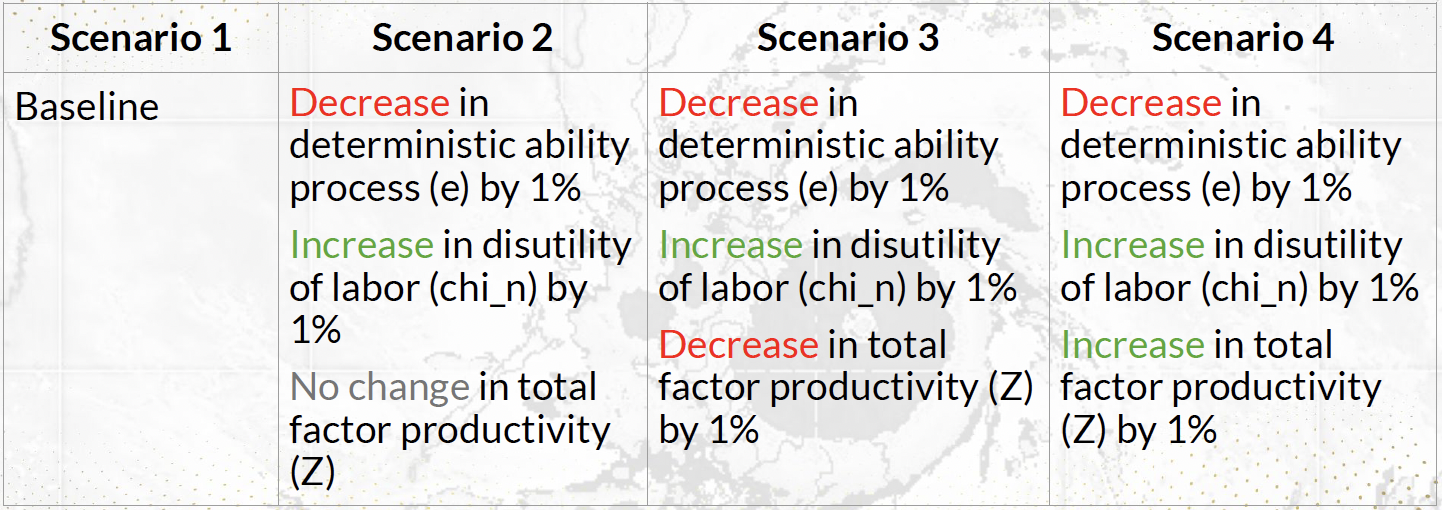
\includegraphics[scale=0.42]{./images/disaster_scenarios.png}
    \end{figure}
  \end{frame}

  \begin{frame}
  \frametitle{Changes in code}
    \begin{figure}[htb]\centering
    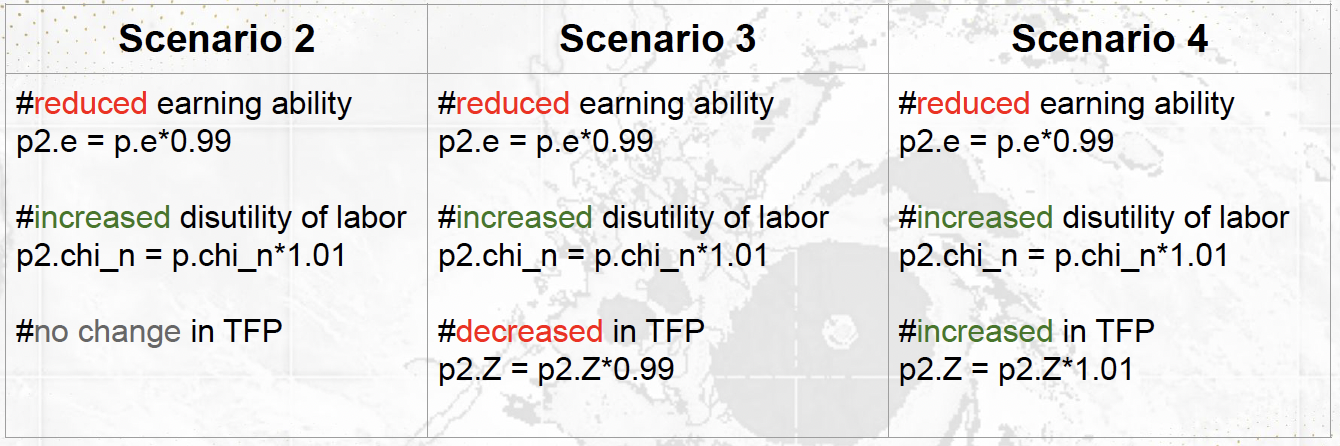
\includegraphics[scale=0.45]{./images/code_changes.png}
    \end{figure}
  \end{frame}

  \begin{frame}
  \frametitle{Scenario 3 output}
    \begin{figure}[htb]\centering
    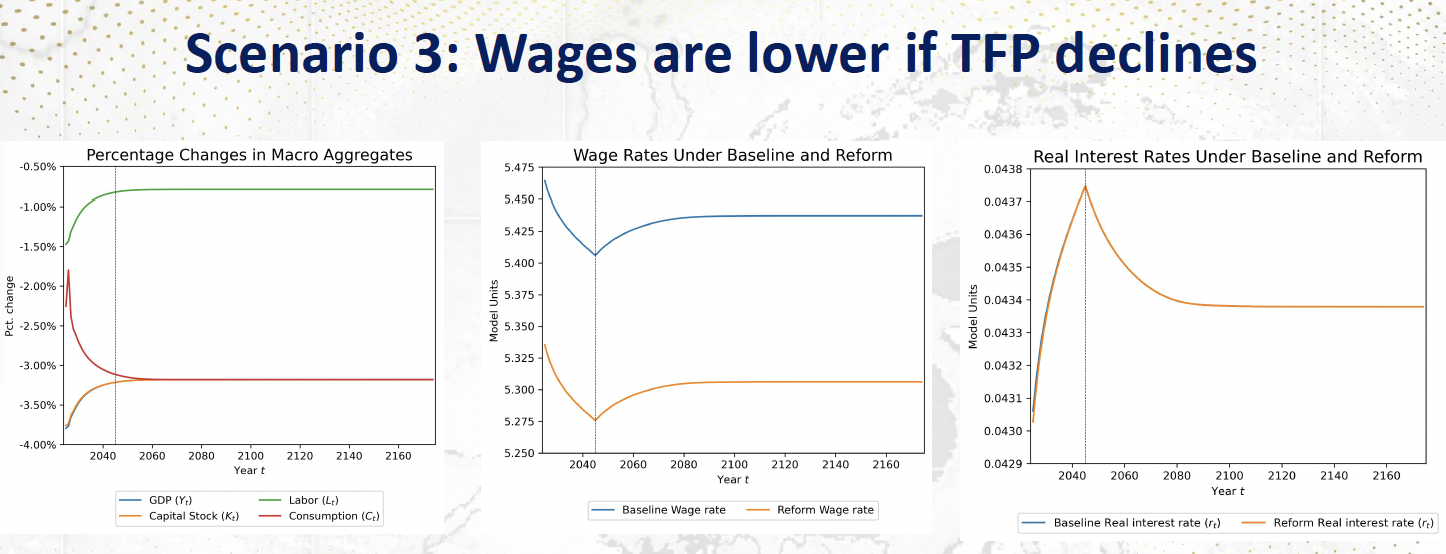
\includegraphics[scale=0.42]{./images/scenario3.png}
    \end{figure}
  \end{frame}

\section{Digitization}

  \begin{frame}
  \frametitle{From 5-day Workshop: August 2024}
    \begin{block}{``Impact of Digitization on the Philippine Economy''}
      Roxanne Elumbre, Kristine Magaling, Clarisa Manzon, Dorothy Obispo
    \end{block}
    \vspace{2mm}
    \begin{itemize}
      \item In the Philippines, the prices of fixed broadband plan is 19.6 percent higher compared with the average price in other ASEAN countries.
      \item Increase productivity of the bottom deciles and reduce capital depreciation
    \end{itemize}
  \end{frame}

\section{Infrastructure investment}

  \begin{frame}
  \frametitle{From 5-day Workshop: August 2024}
    \begin{block}{``Accelerating Government Infrastructure Investments: Boon or Bane?''}
      Arielle Fajardo, FrabertDela Cruz
    \end{block}
    \vspace{2mm}
    \begin{itemize}
      \item ``Build-Better-More'' Program
      \item Increase government investment spending by 5\% of GDP
      \item Financing via debt vs. tax increases
    \end{itemize}
  \end{frame}


\end{document}
